% \title{Trie}
% \author{Ionescu Matei}
% \date{}

% \begin{document}
% \maketitle
\ChapterWithAuthor{Trie}{Ionescu Matei}
\section{Ce este un Trie}

Un trie (sau arbore de prefixe) este un \textit{arbore de căutare k-ar} (un arbore cu rădăcină unde fiecare nod are maxim $k$ fii), reprezentând un mod unic de a memora informațiile, numite și \textit{chei}.

Numărul de fii al unui nod este în mare parte influențat de tipul informațiilor memorate, dar de cele mai multe ori, un Trie este folosit pentru reținerea șirurilor de caractere, astfel fiecare nod având maxim $26$ fii.

Inițial arborele conține doar un singur nod, rădăcina, urmând ca apoi cuvintele să fie introduse în ordinea citirii lor, de la stânga la dreapta. 
Observăm că înălțimea arborelui este lungimea maximă a unui cuvânt.
Complexitatea de timp este \O{\text{lungime maximă}}, iar memoria consumată, în cel mai rău caz, este \O{\text{număr cuvinte} \cdot k}.

\begin{figure}[ht!]
\centering
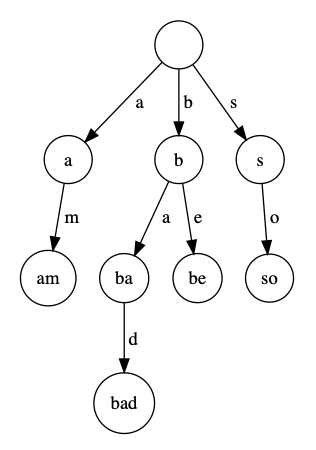
\includegraphics[width=0.5\linewidth]{images/trie/trie.png}
\caption{\label{fig:frog}Un exemplu de trie pentru cuvintele \enquote{am}, \enquote{bad},\enquote{be} și \enquote{so}.}
\end{figure}

\section{Moduri de implementare}
Există două modalități standard prin care putem implementa un Trie, folosind pointeri sau vectori. Ambele funcționează la fel de bine, însă operația de \textit{delete} este mai greu de implementat cu vectori.

\subsection{Prin pointeri}
Ne vom folosi de o structură unde vom reține un contor reprezentând de câte ori am trecut prin nodul curent, cât și un vector de pointeri, reprezentând fiii nodului curent.
\cpp{codes/trie/struct.cpp}

Operația de \textit{insert} poate fi foarte ușor scrisă recursiv.
\cpp{codes/trie/insert_pointeri.cpp}

În momentul în care am ajuns la un nod $node$ în arbore, verificăm dacă există fiul pentru caracterul următor și dacă nu există, îl adăugăm în arbore, apoi apelăm recursiv până ajungem la finalul stringului. 

Pentru a elimina un string din trie ne mai trebuie o informație suplimentară, și anume să știm câți fii are un nod. Așadar, dacă am eliminat un sufix al șirului și nodul curent nu mai are fii nici nu mai este vizitat prin alt șir inserat, putem da erase complet la pointerul respectiv. 
\cpp{codes/trie/del.cpp}

Restul operațiilor se implementează similar, practic baza tuturor operațiilor stă în modul de a parcurge trie-ul.

\subsection{Prin vectori}
În loc de o structură vom folosi un vector cu $k$ coloane. În fiecare element din vector vom reține poziția fiului respectiv.
\cpp{codes/trie/vectori.cpp}

Astfel \textit{trie[node][5]} va fi egal cu poziția în vectorul \texttt{trie} pentru al cincilea fiu a lui $node$.

Operația de \textit{insert} este foarte similară față de cea precedentă, singurul lucru care diferă este modul de implementare. În acest caz ne este mult mai ușor să folosim o funcție care să itereze propriu-zis prin șirul de caractere.
\cpp{codes/trie/insert_vectori.cpp}

Observăm faptul că incrementăm și la final contorul.

\section{Trie pe biți}
Unele probleme necesită reținerea numerelor într-o structură de date, cum ar fi un trie, însa vom înlocui șirurile de caractere cu reprezentarea binară a numerelor.

\subsection{Problema xormax de pe Kilonova (ușoară)}
Un exemplu bun este chiar problema \href{https://kilonova.ro/problems/1984}{xormax}, unde ni se dă un vector cu $N$ elemente și trebuie să aflăm care este suma xor maximă a unui interval. Suma \textsc{xor} a unui interval cu capetele $[L, R]$ este valoarea  $v_L \oplus v_{L+1} \oplus \dots \oplus v_R$, unde $\oplus$ este operatorul \textsc{xor} pe biți.

Pentru a rezolva problema putem parcurge vectorul de la stânga la dreapta și să aflam pentru fiecare $1 \leq i \leq N$ care este suma \textsc{xor} maximă a unui interval care se termină în $i$. Dacă construim vectorul $xp$, unde $xp[i] = v_1 \oplus v_2 \oplus \dots \oplus v_{i-1} \oplus v_i$, atunci suma \textsc{xor} pe intervalul $[L, R]$ este egală cu $xp[R] \oplus xp[L-1]$. Observăm că pentru un $R$ fixat trebuie să găsim care este $L$-ul care maximizează relația de mai sus. Pentru a face asta putem să introducem primii $R-1$ $xp$-uri într-un trie pe biți și să căutăm bit cu bit, începând cu bitul semnificativ, $xp$-ul care va maximiza rezultatul.
\cpp{codes/trie/xormax_solution.cpp}

O variantă care se folosește de implementarea cu pointeri este următoarea:

\cpp{codes/trie/xormax_solution_pointeri.cpp}

\section{Problema \href{https://codeforces.com/contest/1895/problem/D}{XOR Construction} (medie)}
În această problemă ni se dau $n-1$ numere, unde al $i$-lea are valoarea $a_i$, iar noi trebuie să construim alt vector $b$, cu $n$ elemente, astfel încât să existe toate numerele de la $0$ la $n-1$ în $b$, iar $b_i \oplus b_{i+1} = a_i$.

În primul rând, dacă $b_i = 0$ atunci $b_{i+1} = a_i$, $b_{i+1} \oplus b_{i+2} = a_{i+1}$ , deci $b_{i+2} = a_i \oplus a_{i+1}$ și $b_{i+3} = a_i \oplus a_{i+1} \oplus a_{i+2}$. Prin urmare deducem o formă generală pentru $b_j$, unde $i < j$ , și anume $b_j = a_i \oplus a_{i+1} \oplus a_{i+2} \oplus \dots \oplus a_{j-1}$. Proprietatea se respectă și pentru oricare $j < i$, avem $b_j = a_j \oplus a_{j+1} \oplus \dots \oplus a_{i-1}$.

În al doilea rând, enunțul problemei asigură faptul că mereu va exista soluție. Dar când nu avem soluție? Păi în momentul în care se repetă două elemente în vectorul $b$, ceea ce înseamnă faptul că trebuie să existe o secvență cu suma \textsc{xor} egală cu $0$. Pentru simplitate vom spune că pe poziția $k$ va fi $b_k = 0$. Dacă $i < j$ și $b_i = b_j$ și $j < k$, atunci $a_i \oplus a_{i+1} \oplus a_{i+2} \oplus \dots \oplus a_{j-1} = 0$, analog pentru $i > j > k$. Dacă $i < k < j$ și $b_i = b_j$ atunci $b_i = a_i \oplus a_{i+1} \oplus \dots \oplus a_{k-1}$, $b_j = a_k \oplus a_{k+1} \dots \oplus a_{j-1}$. Prin urmare $a_i \oplus a_{i+1} \oplus \dots \oplus a_{j-1} = 0$. Așadar, știm ca mereu în vectorul $b$ elementele vor fi distincte.

În al treilea rând, observăm că vectorul $b$ este generat în funcție de ce valoare are $k$. Deci o primă idee ar fi să fixăm mai întâi unde vom pune $0$-ul în vectorul $b$ și să-l construim în \O{n}, complexitatea temporală fiind \O{n^2}. Dar putem să ne folosim de a doua observație, și anume că mereu vectorul $b$ va avea elementele distincte. Deci ne este suficient să știm care va fi valoarea maximă din $b$ dacă $0$-ul se află pe poziția $k$. Pentru a face asta putem să folosim 2 trie-uri, unul pentru sufix, altul pentru prefix, complexitatea finală devenind \O{n \log n}.

\cpp{codes/trie/sol_xor_constr.cpp}
\section{Problema \href{https://kilonova.ro/problems/65}{cuvinte} (medie-grea)} 
Se dau $N$ cuvinte formate doar din primele $K$ litere mici ale alfabetului englez și un șir $x_i$, de $M$ numere naturale. Trebuie să se formeze $M$ cuvinte astfel încât oricare cuvânt $(1 \leq i \leq M)$ să respecte următoarele proprietăți:
\begin{itemize}
        \item Să aibă lungimea $x_i$.
        \item Să fie format doar din primele $K$ litere mici ale alfabetului englez.
        \item Să nu existe $j \leq M,\, j \neq i$, sau un cuvânt $cuv$ din cele $N$, astfel încât cuvântul $j$ să fie prefix pentru cuvântul $i$, sau $cuv$ să fie prefix pentru $i$.
        \item Să nu existe $j \leq M,\, j \neq i$, sau un cuvânt $cuv$ din cele $N$, astfel încât cuvântul $i$ să fie prefix pentru cuvântul $j$, sau $i$ să fie prefix pentru $cuv$.
\end{itemize}
Prima idee ar fi să sortam vectorul $x$.
Fie $dp_i$ = în câte moduri putem alege primele $i$ cuvinte. Putem considera toate posibilitățile de a forma șirurile , iar abia apoi să vedem cum eliminăm pe cele care nu sunt bune. Cu alte cuvinte, fie $(s_1, s_2, .. , s_{i-1})$ primele $i-1$ cuvinte alese astfel încât să respecte condițiile impuse de problemă. Sunt în total $dp_{i-1} \cdot K^{x_i}$ moduri de a forma un set de șiruri cu primele $i$ cuvinte.

\begin{observation}
Nu există două cuvinte, $s_x$ și $s_y$, astfel încât ambele să fie prefixe pentru $s_i$.
\begin{proof}
Dacă ambele ar fi prefixe pentru $s_i$, atunci fie $s_x$ este prefix pentru $s_y$, fie invers, ceea ce este fals, pentru că noi am generat primele $i-1$ cuvinte optim.
\end{proof}
\end{observation}
Astfel dacă pentru fiecare cuvânt $k$, $k < i$, putem să scădem din numărul total de posibilități șirurile unde $s_k$ este prefix pentru $s_i$, nu vom elimina două configurații la fel.
$dp_i = dp_{i-1} \cdot K^{x_i} - dp_{i-1} \cdot \sum_{j = 1}^{i-1} K^{x_i - x_j}$.

\begin{observation}
Nu există două cuvinte, unul provenit din cele $N$ date și celălalt ($s_k$) din primele $i-1$ astfel încât ambele să fie prefixe pentru $s_i$.
\begin{proof}
Dacă ambele sunt prefixe pentru $s_i$, atunci fie $s_k$ este prefix pentru un cuvânt din cele $N$, fie invers.
\end{proof}
\end{observation}

Deci, putem să fixam un cuvânt din cele $N$ date inițial și să eliminăm numărul de posibilități ca el să fie prefix pentru $s_i$. Datorită observației, nu vom elimina o posibilitate dacă a fost eliminată deja în prima etapă.
În mod natural vom zice că din dp-ul nostru vom scădea în mod similar $dp_{i-1} \cdot \sum_{j = 1}^{N} K^{x_i - len(j)}$, unde $len(j)$ = lungimea cuvântului $j$, cu $x_i \geq len(j)$. Însă nu este adevărat, pentru că dacă avem două cuvinte $x$ și  $y$ , unde $x$ este prefix pentru $y$, atunci suma de mai sus va număra 2 configurații de două ori. Observăm că nouă ne trebuie practic doar acele cuvinte $x$, pentru care nu există alt cuvânt $y$, cu $y$ prefix pentru $x$, iar $len(x) \leq x_i$.
Astfel putem parcurge direct pe Trie-ul cuvintelor. Dacă suntem la un nod $node$, acesta este capătul unui cuvânt, iar $len(cuv) \leq x_i$, atunci putem scădea din dp-ul nostru $dp_{i-1} \cdot K^{x_i - len(cuv)}$ și să oprim parcurgerea. Dacă suntem la un nod $node$, acesta are lungimea egală cu $x_i$, atunci scădem din dp $dp_{i-1}$ și oprim parcurgerea. 

Cu alte cuvinte, o soluție în \O{M^2 + M \cdot S} este posibilă, unde $S = \sum_{i=1}^{N} len(i)$. Putem optimiza soluția, observând că de fiecare dată putem face tranzițiile în \O{1}. Soluția finală devine \O{M + S} sau \O{M \cdot \log + S}. 
\cpp{codes/trie/sol_cuvinte.cpp}
\section{Problema \href{https://kilonova.ro/problems/274}{cli} (medie-grea)}
Se dau $N$ cuvinte care trebuie tastate într-un terminal. Un cuvânt este considerat tastat dacă el va apărea în terminal cel puțin odată pe parcursul tastării. Avem două tipuri de operații la dispoziție: adăugăm un caracter la finalul șirul tastat deja, eliminăm un caracter de la finalul șirului (dacă nu este vid). Pentru fiecare $i = \overline{1, K}$, noi trebuie să aflam care este numărul minim de operații pentru a tasta exact $i$ cuvinte distincte dintre cele date. În momentul în care începem să tastăm un cuvânt, trebuie mereu să începem de la un șir vid\footnote{Voi nota șirul vid cu $\emptyset$. \textit{n.red.}}, și să terminăm tastarea tot la un șir vid. Un exemplu de tastare corectă este: $\emptyset \rightarrow a \rightarrow ab \rightarrow abc \rightarrow ab \rightarrow a \rightarrow \emptyset$.

Ne vom folosi din nou de metoda programării dinamice, dar de data asta vom face dp direct pe trie. Astfel, fie $dp[nod][i]$ = numărul minim de operații pentru a tasta $i$ cuvinte cu prefixul format din lanțul de la rădăcină la $nod$. Acum, pentru un nod fixat din trie-ul nostru, putem presupune că în momentul tastării vom începe mereu cu șirul format de la rădăcină la $nod$, în loc de $\emptyset$. De exemplu, dacă cuvintele au prefixul \textit{abab}, atunci noi vom presupune o succesiune validă de operații: $abab \rightarrow abab\textbf{c} \rightarrow \dots \rightarrow abab\textbf{c} \rightarrow abab$. Putem deci face un rucsac pentru fiii nodului, $dp1[i][j]$ = care e numărul minim de operații pentru a tasta $j$ cuvinte din primii $i$ fii. Pentru că prefixul necesită $\text{len}(prefix)$ operații de adăugare și ștergere, vom începe $dp$-ul nostru cu $2 \cdot \text{len}(prefix)$ operații deja făcute. Cu alte cuvinte, pentru a tasta $0$ cuvinte vom face $dp1[0][0] = 2 \cdot \text{len}(prefix)$.
În momentul în care trecem de la $i$ la $i+1$ avem 2 cazuri: fie nu luăm fiul respectiv în considerare, fie alegem $p$ șiruri pe care le vom tasta în $dp[fiu(i)][p] - 2 \cdot \text{len}(prefix)$ operații. 
\cpp{codes/trie/exemplu_cli.cpp}

Problema constă în faptul că secvența de cod de mai sus rulează pentru fiecare nod din trie, ceea ce ar rezulta într-o complexitate de \O{N \cdot K^2}. Doar că, în practică soluția are complexitatea de \O{N \cdot K}. În momentul în care facem rucsac pe un arbore, este foarte important să fim atenți la memoria și la timpul consumate. Observăm faptul că cele două bucle merg până la $\min(sz[nod], k)$, lucru ce  îmbunătățește timpul de execuție considerabil. Puteți citi mai multe din \href{http://www.lookingforachallengethebook.com/uploads/1/4/5/5/14555448/preview-_looking_for_a_challenge.pdf}{soluția problemei \textit{Barricades}}, iar sursa completă o puteți vizualiza \href{https://kilonova.ro/submissions/140069}{aici}.
\section{Probleme}

\begin{enumerate}
    \item \href{https://kilonova.ro/problems/456}{intervalxor2} (\textit{Trie pe biți persistent. Puteți face queriurile și offline})
    \item \href{https://kilonova.ro/problems/361}{xortree2} (\textit{Problemă \textbf{ok} cu trie pe biți})
    \item \href{https://kilonova.ro/problems/371}{Rps} (\textit{Alt exemplu de dp pe trie})
    \item \href{https://www.infoarena.ro/problema/ratina}{ratina}  (\textit{LCA pe trie})
    \item \href{https://www.infoarena.ro/problema/aiacupalindroame}{aiacupalindroame} (\textit{Nuj ce-i pbma asta, am pus-o că are trie la taguri})
    \item \href{https://www.infoarena.ro/problema/fbsearch}{Facebook Search}  (\textit{Sugestiv numele})
    \item \href{https://codeforces.com/contest/948/problem/D}{Perfect Security}
    \item \href{https://codeforces.com/contest/1902/problem/E}{Collapsing Strings}  (\textit{Dc e asta E?})
\end{enumerate}